% !TEX root = main.tex
%%%%%%%%%%%%%%%%%%%%%%%%%%%%%%%%%%%%%%%%%%%%%%%%%%%%%%%%%%%%%%%%%%%%%%%%%%%%%%%%
% Introduction
%%%%%%%%%%%%%%%%%%%%%%%%%%%%%%%%%%%%%%%%%%%%%%%%%%%%%%%%%%%%%%%%%%%%%%%%%%%%%%%%
\section{Introduction}
\label{section:introduction}

The Cray XK7 Titan supercomputer was the \#1 system in the world for a
very long time, and has remained a critically important computer
system through the end of its life in the Summer of 2019. It defied
scale with 18,688 individual compute nodes and delivered tens of
billions of computing hours to the U.S. Oepartment of Energy
mission-critical programs for nearly 7 years.
 
From a realiability perspective, Titan was a very interesting
machine. Its operation was forced to execute three very significant
rework cycles, two on the mechanical assembly affecting the PCIe
connector from the GPU daughtercard to the motherboard, and a
replacement of about 11,000 GPU assemblies because of a failing
resistor on a printed circuit board. We write primarily about the epoch
that includes this last rework cycle. This includes Titan's most
stable and failure free period and contains the most reliable data on
GPU operation.

Figure~\ref{fig:chronology} illustrates the chronology of the rework
cycles and stable periods as indicated by the number of GPU changes at
periodic inventories.
\begin{figure*}[tbp]
  \centering
  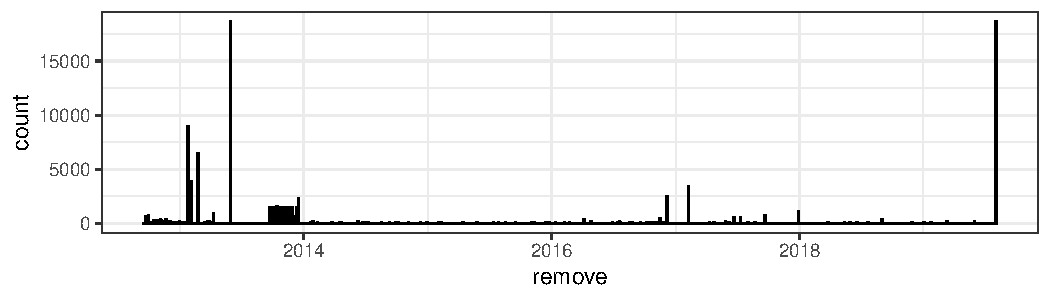
\includegraphics[width=\textwidth]{figs/chronology001.pdf}
  \caption{Daily volume of GPU swaps with labels on most frequent dates.}
  \label{fig:chronology}
\end{figure*}
After an initial fairly stable break-in period, the first rework cycle
begins in early 2013 and ends by May. \fix{Details?}. The second
rework cycle begins in late August of 2013 and ends by mid
December. This is followed by a very long and stable period until
about mid 2016, when GPU failures begin to rise. This results in the
final rework cycle, replacing 11,000 GPUs throughout all of 2017. 

While the 2016 resistor failures were a surprise, there is a known
phenomenon \cite{referenceneeded} that describes a two phase process
that leads to failure. It also explains why there was a very stable
period preceeding the failures. There is specific decay associated
with the electronic components where, as these products age, they will
eventually fail thresholds for guard band margin and other things. In
a lot of cases, they will just fail as well. \fix{Give a reference and
  expand?}

Our analysis focuses on GPUs that were installed in the second rework
cycle and later, essentialy units installed near the beginning of 2014
and later.

We begin by describing related work in Sec.~\ref{section:related}. Our
data collection is desctibed in Sec.~\ref{section:dataprep} and the data
cleaning, checking, and lifetime summarization process in
Sec.~\ref{section:dataclean}. A timme between failures analysis is given
in Sec.~\ref{section:tbf}. Survival analysis based on Kaplan-Meier
modeling and Cox regression modeling of relative hazard rates are in
Sec.~\ref{section:survival}. Finally, we discuss our main conclusions and
recommendations in Sec.~\ref{section:discussion}.
 


